\documentclass[10pt]{beamer}

\usetheme[progressbar=frametitle]{metropolis}
\usepackage{appendixnumberbeamer}

\usepackage{booktabs}
\usepackage[scale=2]{ccicons}

\usepackage{pgfplots}
\usepgfplotslibrary{dateplot}

\usepackage{xspace}
\newcommand{\themename}{\textbf{\textsc{metropolis}}\xspace}

\title{Scanner, parser, and pretty-printer in Rust}
\subtitle{Compiler Construction presentation}
\date{}
\author{Oussama Danba}

\begin{document}

\maketitle

\begin{frame}{Table of contents}
  \setbeamertemplate{section in toc}[sections numbered]
  \tableofcontents[hideallsubsections]
\end{frame}

\section{Why Rust?}
\begin{frame}{Why Rust?}
    \begin{itemize}
    \item Not enough confidence programming in functional languages
        \begin{itemize}
            \item Rust still has a lot of features from functional languages
        \end{itemize}
    \item Easy crate/library usage
    \item Low-level imperative language with a lot of guarantees through the typing system (and static analysis)
    \item Personal preference and a good opportunity to gain experience using a larger project
        \begin{itemize}
            \item Anything that I can do in other languages I can do in rust (with more work)
        \end{itemize}
\end{itemize}
\end{frame}

\begin{frame}{Disadvantages of Rust}
    \begin{itemize}
        \item Recursive data structures difficult
            \begin{itemize}
                \item Will not compile unless the size of the type is known at compile-time
            \end{itemize}
        \item Build times slow (especially on larger projects)
        \item Verbose at times
    \end{itemize}
    
    \metroset{block=fill}
      \begin{block}{Mapping some string to a Token}
        fn recognize\_symbol<'a>(input: \&'a str, recognizer: \&str, token: Token) -> Option<(Token, \&'a str)>
      \end{block}
\end{frame}

\section{Compiler structure}
\begin{frame}{General structure}
    \begin{itemize}
        \item Loading in file / preprocessing
            \begin{itemize}
                \item Checks if input file exists and such
            \end{itemize}
        \item Scanner/Lexer
        \begin{itemize}
            \item Goes from a string to a vector/list of tokens
        \end{itemize}
        \item Parser
        \begin{itemize}
            \item Goes from a vector of tokens to an AST
        \end{itemize}
        \item Pretty-printer
        \begin{itemize}
            \item Outputs a formatted AST
        \end{itemize}
    \end{itemize}
\end{frame}

\section{Scanner}
\begin{frame}{Scanner}
    Works recursively by scanning a token and then calling scan on the rest of the input.

    \metroset{block=fill}
    \begin{block}{Scanning}
        pub fn scan(input: \&str) -> Result<Vec<(Token, usize)>, usize>
      \end{block}
    Returns a list of tokens and their position or the position where a scanner error occurred.
\end{frame}

\begin{frame}{Example recognizer}
    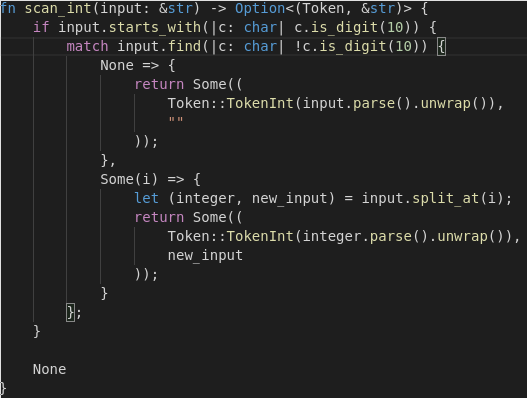
\includegraphics[width=\textwidth]{scan_int.png}
\end{frame}

\begin{frame}{Example error output}
    \metroset{block=fill}
    \begin{block}{Given program}
    main() :: -> Void \{\\
        \hspace{1cm} return`;\\
    \}
    \end{block}
    Returns the error:
    \metroset{block=fill}
    \begin{block}{}
    Scanner error at line 2 near `:\\
        \hspace{1cm} return`;
    \end{block}
\end{frame}

\begin{frame}{Example correct output}
    \metroset{block=fill}
    \begin{block}{Given program}
    main() :: -> Void \{\\
        \hspace{1cm} return;\\
    \}
    \end{block}
    Returns the following vector/list:
    \metroset{block=fill}
    \begin{block}{}
    [(TokenIdentifier("main"), 0), (TokenParenOpen, 4), (TokenParenClose, 5), (TokenDoubleColon, 7), (TokenArrow, 10), (TokenVoid, 13), (TokenBraceOpen, 18), (TokenReturn, 24), (TokenSemiColon, 30), (TokenBraceClose, 32)]
    \end{block}
\end{frame}

\begin{frame}{Miscellaneous}
    Scanning is fairly straightforward. The most significant choice was not scanning negative numbers immediately.
    \metroset{block=fill}
    \begin{block}{Might produce parsing error}
    return (5 -4);
    \end{block}
    Scanner is about 230 lines of code.
\end{frame}

\section{Parser}
\begin{frame}{General parser information}
    \begin{itemize}
        \item Goes from a list of tokens to an AST iff valid program was given
        \item Makes use of parser combinators (and is thus a top-down parser)
            \begin{itemize}
                \item Using the combine crate
            \end{itemize}
        \item About 400 lines of code excluding the AST type definition
        \item Able to report parsing errors in a similar way to scanner errors
    \end{itemize}
\end{frame}

\begin{frame}{Combine crate}
    \begin{itemize}
        \item Modeled after parsec (from Haskell).
        \item Allows to use parser combinators in Rust.
        \item Mostly intended to work on characters rather than tokens so I had to reimplement some small combinators.
        \item Documentation lacking (mostly examples). Spent a day figuring everything out.
        \begin{itemize}
            \item Library abstract a lot of typing information away making it difficult sometimes
        \end{itemize}
    \end{itemize}
\end{frame}

\begin{frame}{Example parser}
    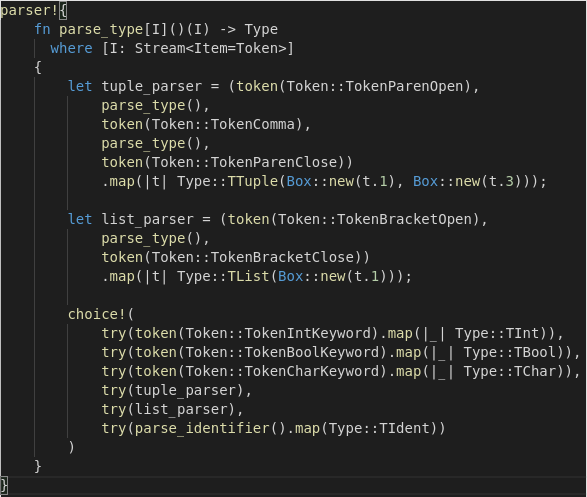
\includegraphics[width=\textwidth]{parse_type.png}
\end{frame}

\begin{frame}{Solving left-recursion and associativity}
    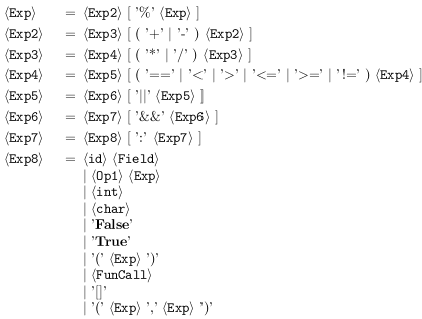
\includegraphics[width=\textwidth]{grammar.png}
\end{frame}

\section{Pretty-printer}
\begin{frame}{General pretty-printer information}
    \begin{itemize}
        \item AST implements the Display trait. Much like implementing + on a custom type.
            \begin{itemize}
                \item format("\{\}", ast);
            \end{itemize}
        \item Supports indenting and does not produce (too many) superfluous parenthesis
        \item About 180 lines of code (a lot of pattern matching!)
    \end{itemize}
\end{frame}

\begin{frame}{Example implementation of Display trait}
    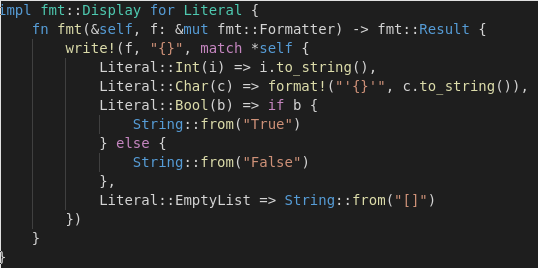
\includegraphics[width=\textwidth]{literal.png}
\end{frame}

\begin{frame}{Example pretty print (output can be used as input again!)}
    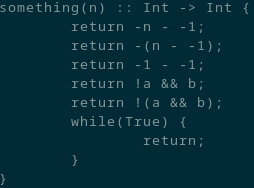
\includegraphics[width=\textwidth]{pretty_printed.png}
\end{frame}

\section{Ending}
\begin{frame}{Current status}
    \begin{itemize}
        \item Scanner and parser are complete and shouldn't need any significant changes (hopefully)
    \item Didn't run into too many problems but did take quite some time to program
    \item Happy with the code so far
        \begin{itemize}
            \item Not sure if I would go the same route again since compilation time has exploded by using parser! macros.
        \end{itemize}
    \end{itemize}
\end{frame}

{\setbeamercolor{palette primary}{fg=black, bg=yellow}
\begin{frame}[standout]
  Questions?
\end{frame}
}

\begin{frame}{License information}

  Get the source of this theme from

  \begin{center}\url{github.com/matze/mtheme}\end{center}

  The theme \emph{itself} is licensed under a
  \href{http://creativecommons.org/licenses/by-sa/4.0/}{Creative Commons
  Attribution-ShareAlike 4.0 International License}.

  \begin{center}\ccbysa\end{center}

\end{frame}

\end{document}
